\newpage
\section{Hintergrund und theoretische Grundlagen}

Mechanische Neuronale Netzwerke (MNNs) scheinen künstlichen neuronalen Netzwerken (\eng{artificial neural networks}, kurz ANNs) in ihrem Aufbau zwar ähnlich (vgl. Abb. \ref{fig:dense_nn} und \ref{fig:mnn2-1}), unterscheiden sich in ihrer Funktionsweise und Umsetzung jedoch stark.

\begin{figure}[H]
    \def\layersep{6cm}
    \def\biasDist{0.6}
    \centering
    \adjustbox{scale=0.9}{%
    \begin{tikzpicture}[
        % scale=1.2,
        shorten >=1pt,->,draw=black!70, node distance=\layersep,
        neuron/.style={circle,fill=black!25,minimum size=20,inner sep=0},
        edge/.style 2 args={pos={(mod(#1+#2,2)+1)*0.33}, font=\tiny},
        distro/.style 2 args={
            edge={#1}{#2}, node contents={}, minimum size=0.6cm, path picture={\draw[double=orange,white,thick,double distance=1pt,shorten >=0pt] plot[variable=\t,domain=-1:1,samples=51] ({\t},{0.2*exp(-100*(\t-0.05*(#1-1))^2 - 3*\t*#2))});}
          },
        weight/.style 2 args={
            edge={#1}{#2}, node contents={\pgfmathparse{0.35*#1-#2*0.15}\pgfmathprintnumber[fixed]{\pgfmathresult}}, fill=white, inner sep=2pt
          }
      ]
    % Input layer
    \foreach \y in {1,...,2}
        \node[neuron, fill=green!40] (i\y) at (0,\y+1) {$i_\y$};
    \node[neuron, fill=orange!40, above=\biasDist of i2] (b1) {$b_1$};
    % Hidden layer
    \foreach \y in {1,...,4}
        \path node[neuron, fill=blue!40] (h\y) at (\layersep,\y) {$h_\y$};
    \node[neuron, fill=orange!40, above=\biasDist of h4] (b2) {$b_2$};
    % Output node
    \node[neuron, fill=red!40] (o) at (2*\layersep,2.5) {$O$};
    
    % Connect every node in the input layer with every node in the hidden layer.
    \foreach \source in {1,...,2}
        \foreach \dest in {1,...,4}
            \path (i\source) edge (h\dest);
    % Connect bias in the input layer with every node in the hidden layer.
    \foreach \dest in {1,...,4}
        \path[red!20] (b1) edge (h\dest);
    % Connect every node in the hidden layer with the output layer
    \foreach \source in {1,...,4}
        \path (h\source) edge (o);
    % Connect bias in the hidden layer with the output layer
    \path[red!20] (b2) edge (o);
        
    % Draw weights for all regular edges.
    \foreach \i in {1,...,2}
        \foreach \j in {1,...,4}
            \path (i\i) -- (h\j) node[weight={\i}{\j}];
    \foreach \i in {1,...,4}
        \path (h\i) -- (o) node[weight={\i}{1}];
    % Draw weights for bias edges.
    \foreach \j in {1,...,4}
        \path (b1) -- (h\j) node[weight={3}{\j}];
    \path (b2) -- (o) node[weight={5}{1}];
    \end{tikzpicture}
    }
    \caption{Ein Beispiel für ein neuronales Netzwerk bestehend aus einer Eingabeschicht($i_1$ und $i_2$) und zwei vollständig verbundene Schichten (Neuronen $h_1$ bis $h_4$ mit Bias $b_1$ und Neuron $O$ mit Bias $b_2$). 
    Die Kreise stellen Neuronen dar; die Zahlen auf den Pfeilen die Gewichte zwischen den jeweiligen Neuronen.}
    \label{fig:dense_nn}
\end{figure}

Die von \lee{} vorgeschlagene Architektur besteht aus drei Komponenten: zwei fixierten und parallelen Wänden sowie miteinander verbundenen Federn, welche in gleichseitigen Dreiecken angeordnet sind  (s. Abb. \ref{fig:mnn2-1}, links).
Die gleichseitigen Dreiecke wurden aufgrund ihres höheren Trainingserfolgs gegenüber Quadraten gewählt (vgl. \cite[Abb. 5]{Lee2022}).
Wir nennen die Knotenpunkte zwischen Federn sowie Befestigungspunkte an den \enquote{Wänden} äquivalent zu ANNs Neuronen.
Dabei sollte noch einmal klar gestellt werden, dass die Knotenpunkte keine echten Neuronen sind, sondern Massepunkten eines mechanischen physikalischen Systems entsprechen.
Durch die Fixierung der äußeren Neuronen auf zwei gegenüberliegenden Seiten durch die Wände wird die Bewegung der Federn so eingeschränkt, dass es eine klare Eingabe auf der einen Seite und Ausgabe auf der anderen gibt.

Während ANNs nur rein mathematische Konstrukte sind, sind MNNs physisch, was Vor- und Nachteile mit sich bringt. 
% Datenverarbeitung relevant?
So eignen sich MNNs nicht für Datenverarbeitung, u.a. aufgrund der Begrenzung auf hier zwei, maximal drei Dimensionen und, wie später noch beschrieben wird, stellt die technische Umsetzung ebenfalls Schwierigkeiten dar.
Doch sie bieten als analoges System einen großen Vorteil: Während ANNs für die Evaluierung von Eingaben Zeit und Ressourcen benötigt, funktionieren trainierte MNNs ohne signifikante Verzögerung.

Gegenüber \enquote{konventionellen} Materialien bieten sie zwei hauptsächliche Vorteile:

\begin{enumerate}
    \item Es können mehrere Verhaltensweisen auf externe Kräfte gleichzeitig antrainiert werden.
    \item Bei der Implementation von \lee{} kann das MNN durch Sensoren auch beim Einsatz weiterlernen, sodass es sich von selbst an Beschädigung oder Abnutzungen, Größenänderung usw. anpassen kann.
\end{enumerate}

%Doch beim aktuellen Stand der Technik 

%Denn bei MNNs beeinflussen sich mehr Neuronen untereinander und die Simulation / Ausführung ist sehr langsam. Letzteres ist unter anderem dadurch verantwortet, dass eine manuelle Ableitung der Positionen der Neuronen nach der Stabilisierung in Abhängigkeit der Gewichte in einem MNN nur schwer machbar wäre.

% Zum einen gibt es durch die physische Simulation gibt es nicht eine Richtung: Neuronen einer Schicht können Einfluss auf Neuronen der davon linken Schicht nehmen.
% Außerdem ist der Forwardpass deutlich komplexer.
% - schwierige manuelle Ableitung
% - Performance

%Es gibt eine darauf aufbauende Arbeit von Hopkins et al. (vgl. \cite{Hopkins2023}), welche \eng{binary-stiffness beams} verwendet, also Federn zwischen den Neuronen, welche anstelle einer beliebigen Steifheit zwischen zwei Grenzwerten nur zwischen zwei verschiedenen wechseln können -- einem möglichst niedrigem und einem hohen.
%Die Verwendung von \eng{binary-stiffness} Federn bietet hauptsächlich zwei Vorteile: Schnelleres Trainieren bei gleicher Netzwerkgröße mit Verfahren wie PPS und evolutionärem Training aufgrund der niedrigeren Anzahl an möglichen Kombinationen sowie eine einfachere physische Umsetzung.
%Letzteres beinhaltet, je nach Umsetzung, einen niedrigeren bis nicht-existenten Energieverbrauch außerhalb des Trainings sowie eine einfachere Verkleinerung des Systems und weniger Kontrolltechnik.

%Jedoch bieten sie einen großen Nachteil: Durch das Fehlen von negativen Steifheiten sowie die Begrenzung der annehmbaren Steifheiten sind deutlich mehr Federn und vor allem Schichten an Federn nötig, um komplexe Probleme ähnlich gut lösen zu können wie die von \lee{} vorgeschlagene Architektur. %TODO: Vorher Nennung Lee

%Da der Transfer der Bewegung von einem zum anderen Ende jedoch komplett passiv verläuft führt dies zu einem deutlich stärkeren \enquote{Verbrauch} der kinetischen Energie, sodass die einwirkenden Kräfte deutlich höher sein müssen, um den Effekt an der anderen Seite ebenso sehen zu können.

\subsection{Simulation von MNNs}

Da ein MNN nur aus miteinander verbundenen Federn besteht, lässt sich die Kraft, die auf jedes Neuron wirkt, durch die Summe aller einzelnen Kräfte, die jede Feder auf das Neuron ausübt, beschreiben.
Um diese einzelnen Kräfte zu bestimmen, benötigt man eine Funktion, die mithilfe der Auslenkung (Entfernung von der Ruhelage) und der Steifheit der Feder (Federkonstante) die Kraft bestimmen kann.
Hierfür wird oft das Hooke'sche Gesetz genutzt, welches die Kraft $F$ als Produkt von Federkonstante $k$ und Auslenkung $x$ angibt \cite{wiki:hooke}. Es gilt also:

{\[
    F = -k *  x
    %F = -k x
\]}

Um nun mit der Formel für die Kraft, die auf die Neuronen wirkt, die Position dieses Neuronen als Funktion der Zeit angeben zu können, um das Verhalten des MNNs unter verschiedenen Krafteinflüssen zu analysieren, muss man die obige Formel 
mithilfe des Newton'schen Gesetzes
zu einer Differenzialgleichung für die Beschleunigung des Neurons ($m \ddot x $) umwandeln.
%man F durch  ersetzt. Die Lösung dieser Differenzialgleichung ist dann die gesuchte Funktion. 
Im einfachsten Fall, für ein einzelnes bewegliches Neuron und eine Feder, ergibt sich die Gleichung 

{\[
m \ddot{x} = -k x
\]}


Diese Gleichung kann nun von einem Computerprogramm numerisch gelöst werden. Dafür haben wir das Package DifferentialEquations.jl verwendet.
Um die Ergebnisse zu validieren, wurden die Gleichungen zusätzlich noch nach einem selbst programmierten Eulerverfahren gelöst.
Dabei addieren wir jeweils in sehr kurzen Zeitabständen das Produkt der berechneten Beschleunigung und des Zeitabstandes zu der Geschwindigkeit jedes Neurons hinzu und aktualisieren die Positionen aller Neuronen mithilfe der berechneten Geschwindigkeiten.

Zusätzlich muss noch eine Änderung durchgeführt werden, die es ermöglicht, den Ruhezustand des Systems bei bestimmten Krafteinflüssen zu ermitteln.
Damit das MNN überhaupt einen Ruhezustand erreichen kann, muss es gedämpft werden.
Ohne diese Dämpfung würde das Netzwerk einfach immer weiter schwingen. 
Die Dämpfung lässt sich durch einen zusätzlichen Term $-\gamma \dot{x}$ beschreiben, also als das Produkt aus 
Dämpfungskonstante $\gamma$ und der
%(größer als 0 und kleiner als 1) beschreiben, mit dem man die 
Geschwindigkeit $\dot{x}$ jedes Neurons.
%multiplizieren muss, 
Durch diese Kraft werden die Neuronen abgebremst.

Jedoch können MNNs, welche nur positive Federkonstanten besitzen, nicht alle möglichen Verhaltensweisen lernen, da sie nur Kräfte durch das Material \enquote{transportieren}.
Wenn zum Beispiel eine Kraft, welche nach rechts ausgerichtet ist, auf ein MNN trifft, werden sich alle Neuronen des MNNs nach rechts bewegen (s. Abb. \ref{fig:positive_springs}).
Um auch Verhalten, welche Bewegung entgegen einer Kraft benötigen, umzusetzen, muss dem System Energie zugefügt werden. Dies lässt sich mit negativen Federkonstanten umsetzen. 
Federn mit negativen Federkonstanten stoßen Neuronen, die sich weit von einander entfernt befinden, ab und ziehen nahe Neuronen noch weiter an (s. Abb. \ref{fig:force}).
Jedoch sind MNNs mit negativen Federkonstanten nicht stabil, da es zum Beispiel passieren kann, dass sich zwei durch eine Feder mit negativer Federkonstante verbundene Neuronen voneinander entfernen, wodurch sie sich weiter abstoßen würden, wodurch sie sich weiter voneinander entfernen.
Um so einen Kreislauf zu verhindern und um die Stabilität des MNNs zu gewährleisten, muss von einem linearen Verhältnis von Kraft und Distanz abgewichen werden.
Es muss eine Auslenkung geben, bei welcher die Kraft, die auf die Neuronen wirkt, auch bei negativen Federkonstanten entgegen der Richtung des Auslenkungsvektors wirkt (s. Abb. \ref{fig:force}). In diesem Projekt wurde dafür eine Funktion dritten Grades gewählt:

{\[
    %F(\Delta x) = -k * \Delta x -  \Delta x^3
    F(x, k) = -k *  x -  x^3
\]}

\begin{figure}[H]
    \centering
    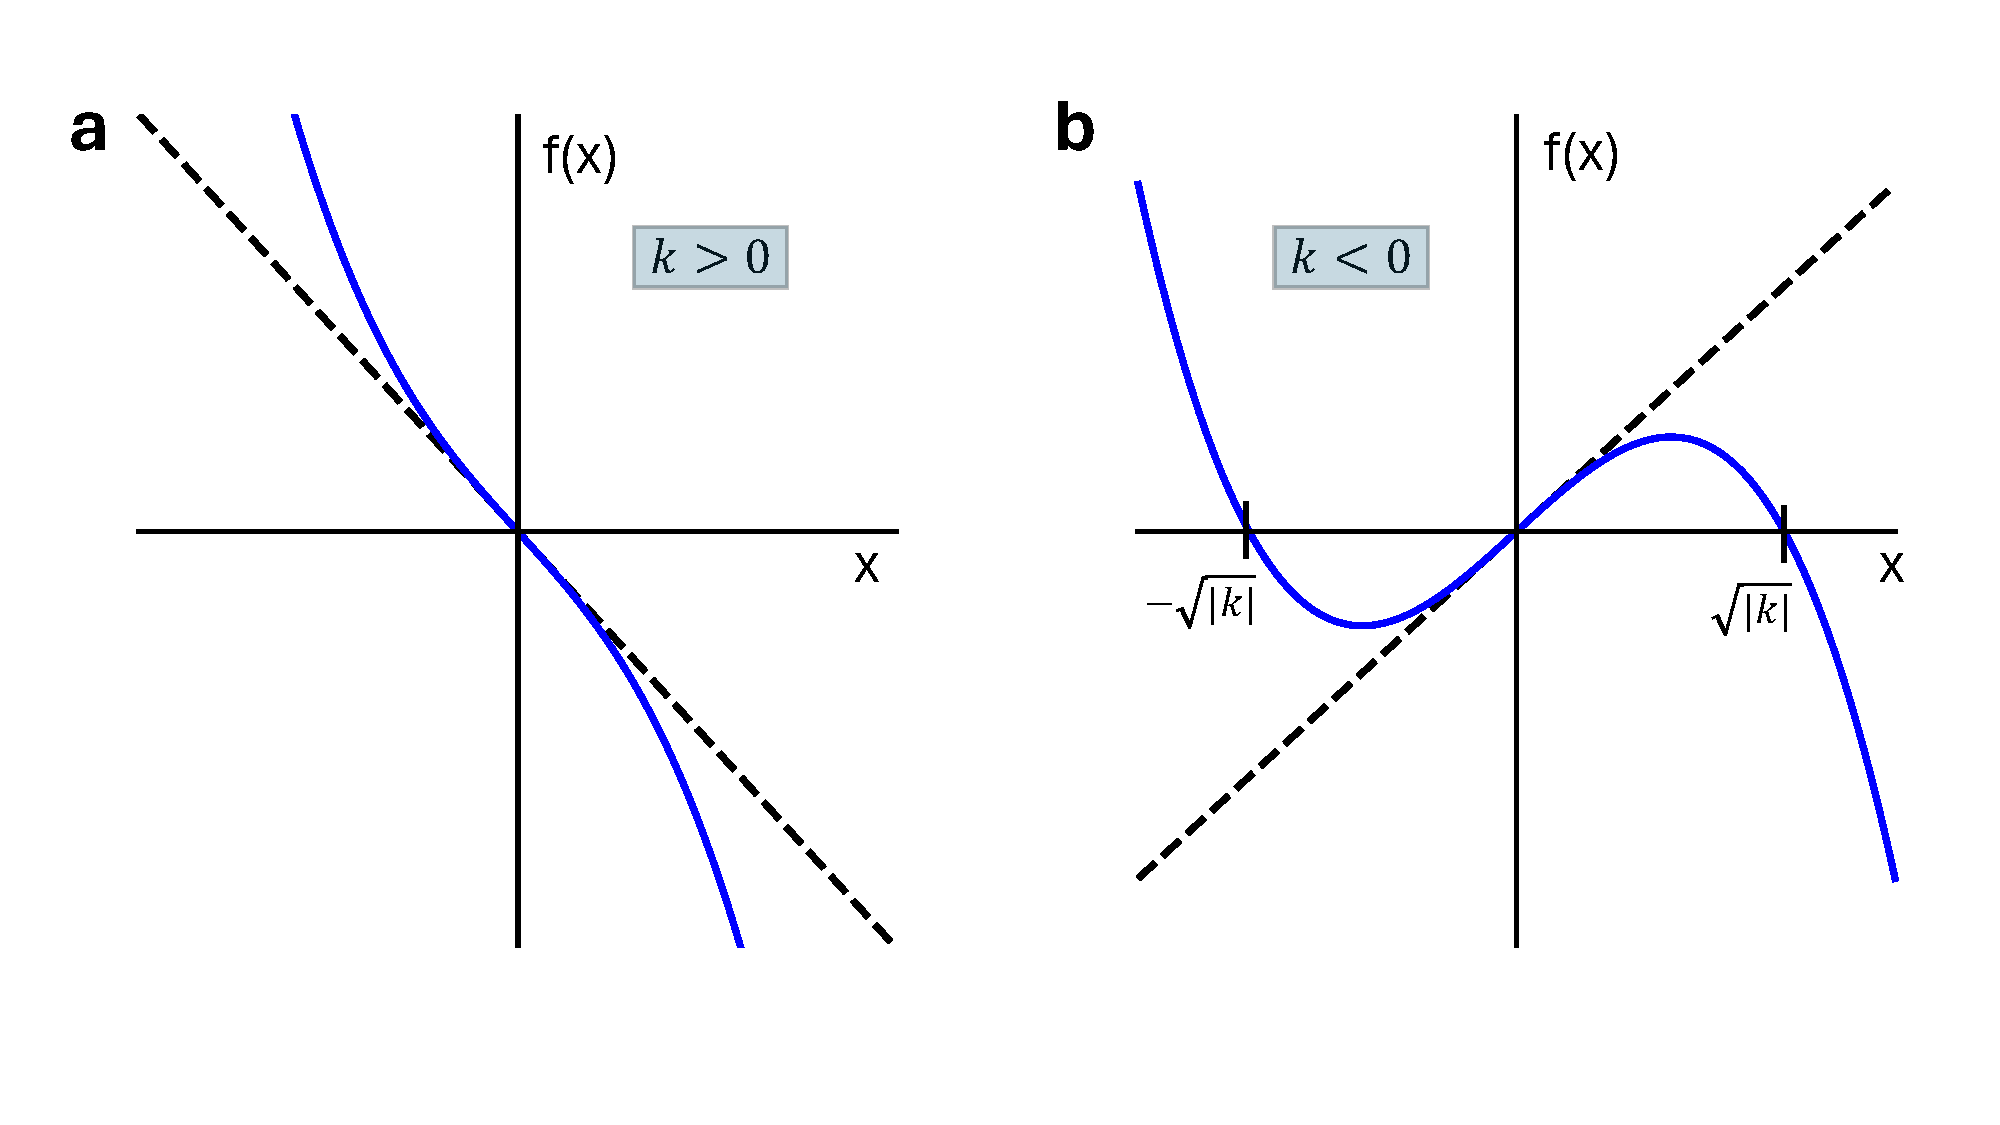
\includegraphics[width=0.8\linewidth]{bilder/kraft.pdf}
    \caption{Skizze der verwendeten Federkraft $f(x)$ in
    Abhängigkeit der Auslenkung $x$ für den Fall einer positiven
    Federkonstante $k>0$ (links) und einer negativen Federkonstante $k<0$
    (rechts). Die gestrichelte Linie zeigt einen linearen Kraftverlauf
    $f(x) = -kx$.  Im Falle einer positiven Federkonstante (links)
    entspricht dies dem Hooke'schen Gesetz und führt zu einem stabilen
    Gleichgewicht, da eine positive Auslenkung der Feder zu einer
    negativen Kraft führt und umgedreht. Im Falle einer negativen
    Federkonstante ist das Gleichgewicht $x=0$ instabil und eine leichte
    Auslenkung der Feder führt zu einer unendlich großen Auslenkung. Um
    diese Instabilität zu vermeiden, verwenden wir die Kraft $f(x) = -kx -
    x^3$ (blaue durchgezogene Linie). Im Falle von $k>0$ führt dies zu
    einem leicht nichtlinearen Kraftverlauf, aber immer noch stabilem
    Gleichgewicht (links). Für $k<0$ ist das Gleichgewicht immer noch
    instabil, aber für große Auslenkungen $|x| > \sqrt{|k|}$ wirkt die
    Kraft stabilisierend}
    \label{fig:force}
\end{figure}

\begin{figure}[h!]
    \centering
    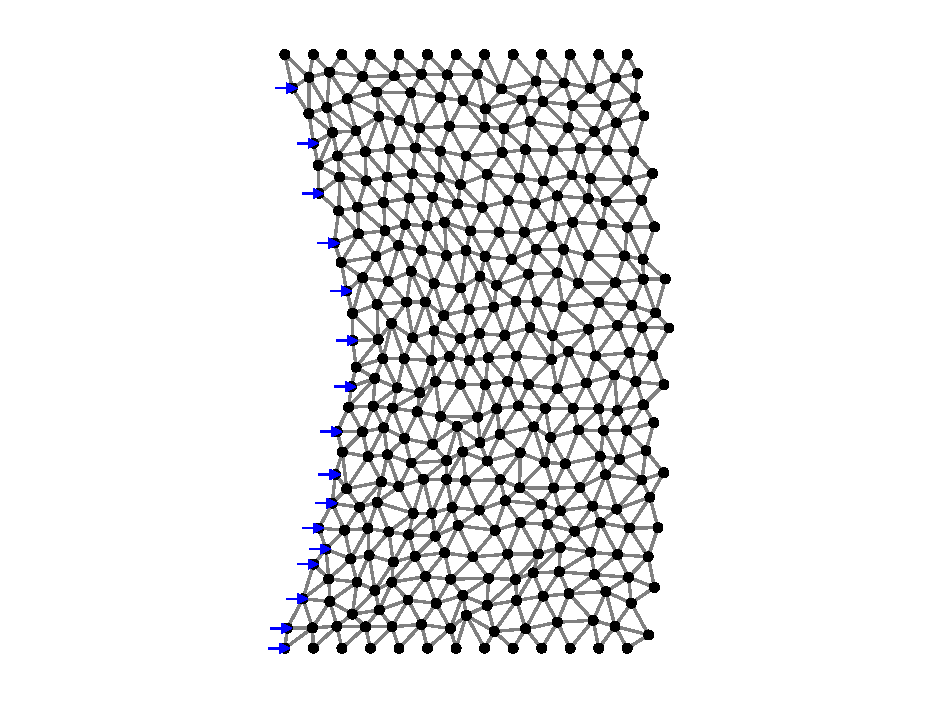
\includegraphics[trim=0cm 0.8cm 0cm 0.8cm, clip]{bilder/test4.pdf}
    \caption{Typischer Aufbau eines MMNs. Dieses besteht aus Neuronen (schwarze Kreise), die durch Federn (schwarze Linien) verbunden sind. Die Neuronen am oberen und unteren Ende sind mechanisch fixiert und können sich nicht bewegen.
    Die blauen Pfeile stellen die Krafteinwirkung auf die Neuronen dar.
    %Abbildung eines MNNs mit positiven Federkonstanten, auf das eine Kraft nach rechts ausgeübt wird.
    }
    \label{fig:positive_springs}
\end{figure}

Da wir die MNNs jedoch im 2-dimensionalen Raum simulieren wollen, müssen wir die Beschleunigung auch als 2-dimensionalen Vektor angeben, indem wir die Kraft noch mit einem normierten Richtungsvektor multiplizieren, der die Richtung der Feder und demnach auch der Kraft beschreibt. 
Weiterhin müssen alle Kräfte, die auf ein Neuron wirken, aufsummiert werden.
Die vollständige Differenzialgleichung lautet also:

{\[
    m \ddot{\vec{x}}_{i} = \sum_{j \in \textrm{NN}(i)} \left( F\left(\Delta x_{ij} - l, k_{ij}\right)
     * \frac{\vec{\Delta x_{ij}}}{ \Delta x_{ij}} \right)
     - \gamma \dot{\vec{x}}_i + \vec{F}_{\textrm{ext}, i}
\]}

Hier ist $ \vec{\Delta x}_{ij} = \vec{x}_i - \vec{x}_j$, also der Abstandsvektor zweier Neuronen,
$\Delta x_{ij}= \| \vec{\Delta x}_{ij} \|$, $l$ die Ruhelänge der Feder, 
$\vec{F}_{\textrm{ext}, i}$ die externe Kraft auf Neuron $i$ und die Summe läuft über die nächsten Nachbarn $j = \textrm{NN}(i)$ des Neurons. 

%{\[
%    \ddot x = \sum k * \Delta x * \frac{\vec{v}}{\| \vec{v} \|}
%\]}
%Die vollständige Differenzialgleichung lautet also:


%{\[
%    \ddot x_{i} = \sum_{j \in \textrm{neighbors(i)}} (-k * \Delta x -  \Delta x^3) * \frac{\vec{v_{ij}}}{\| \vec{v_{ij}} \|}
%\]}

\subsection{Optimierungsverfahren von MNNs}

Um ein MNN zu optimieren, benötigt man zuerst einmal einen Trainingsdatensatz an verschieden Verhaltensweisen, welche erlernt werden sollen. In unserem Fall besteht ein Verhalten aus den Kräften, die auf die Neuronen in der ersten Schicht wirken, und die Änderungen der Positionen der Neuronen in der letzten Schicht, die durch die gegeben Kräfte bewirkt werden sollen. Mithilfe eines Trainingsdatensatzes lässt sich nun auch bestimmen, wie gut ein Modell die Verhaltensweisen umsetzt, indem man die Entfernung jedes Neurons zu den in den Trainingsdaten gegebenen Positionen berechnet und für alle Neuronen aufsummiert. Man berechnet also die Abweichungen der Neuronen zu den Trainingsdaten. Zuletzt wird diese Abweichung noch quadriert. Diese Verfahren nennt sich \feng{mean squared error} (MSE).

\subsubsection{Genetische Algorithmen}

Genetische Algorithmen können MNNs optimieren, indem sie sich an Ideen der Evolution orientieren \cite{gentisch}. Mehrere MNNs bilden eine Population ab.
Der genetische Algorithmus beginnt damit, jedem MNN der Population einen \feng{score} zu geben, welcher beschreibt, wie gut dieses MNN die Trainingsdaten abbilden kann. Das Ziel ist es, diese Zahl zu minimieren.
Die besten MNNs werden ohne Mutation direkt an die nächste Generation übergeben.
Anschließend wird der Rest der folgenden Population durch \feng{crossover} bestimmt. Dies funktioniert, indem zwei MNNs aus der Population ausgewählt werden, wobei bessere MNNs eine höhere Wahrscheinlichkeit haben, ausgewählt zu werden.
Die Federkonstanten der beiden ausgewählten MNNs werden beim \feng{crossover} genutzt, um ein neues MNN zu erstellen, das Federkonstanten beider \enquote{Elternteile} besitzt.
Am Ende einer Iteration werden noch zufällige Mutationen vorgenommen. Die Stärke dieser Mutation nennt sich Lernrate.
Dieses Verfahren wird solange wiederholt, bis ein zufriedenstellendes MNN gefunden wurde.

\subsubsection{Partial Pattern Search}

Bei dem von \lee{} verwendeten \feng{partial pattern search} (PPS) Verfahren werden zu Beginn alle Federkonstanten auf den gleichen voreingestellten Wert gesetzt, hierfür  haben wir den von \lee{} verwendeten Wert von \num{1,15} %TODO: Einheit
übernommen.
Weiter gibt es zu Beginn eine festgesetzte Änderungsrate von 1.
Nun wird in zufälliger Reihenfolge zu jeder Federkonstante die aktuelle Änderungsrate addiert. Falls der MSE mit der veränderten Federkonstante nicht niedriger ist als vorher, wird die Änderung rückgängig gemacht.
Sollte es in einem Durchlauf aller Federkonstanten keine Verbesserung des MSE gegeben haben, wird das Vorzeichen der Änderungsrate umgekehrt und, falls diese bereits negativ war, um \SI{10}{\percent} gesenkt. Mit den genannten Werten wäre die Entwicklung der Änderungsrate also $1 \rightarrow -1 \rightarrow 0.9 \rightarrow -0.9 \rightarrow 0.81 \dots$
Dies wird für eine vorgegebene Anzahl an Wiederholungen durchgeführt, wobei eine Wiederholung nicht einen Durchlauf aller Federkonstanten, sondern die Anwendung der aktuellen Änderungsrate auf eine einzelne Federkonstante bezeichnet.